\section{Design of the proposed attacks} \label{sec:design_attacks}
%%%%%%%%%%%%%%%%%%%%%%%%%%%%%%%%%%%%%%%%%%%%%%%%%%%%%%%%%%%%%%%
In this section, we present a number of novel concepts aimed towards improving and extending label flipping techniques. To push the limits of effectiveness and applicability, each hypothesis is motivated by a strategic vision that combines theoretical insights with practical considerations.

\subsection{Main structure of the hypotheses code}
In order to test our hypotheses, we first have to design how the code will be structured. The main idea is to have an if-statement for each hypothesis inside the \textit{participant\_update()} function, which is called each time a peer has to train and send the local model to the server. This condition will contain all the code needed to perform the label flipping attack. The code will be structured as follows:
\begin{enumerate}
        \item The first step is to iterate through the local model's samples.
                \begin{enumerate}
                        \item For each sample, we have to check if the sample's label is the source class's label. If it is, we must keep its index in a list.
                        \item After that, we have to make any calculation needed in order to obtain some kind of punctuation to give to each sample. This punctuation will be used to determine which samples will be flipped.
                \end{enumerate}
        \item Joining the index list with the punctuation list. This is helpful because we can sort the list by the punctuation and then flip the labels of the samples with the highest punctuation.
        \item Determining which samples to flip based on the punctuation obtained in the previous step.
        \item Flipping the labels of the samples selected in the previous step, given their indices.
        \item Loading the new dataset with the flipped labels into the dataset used to train the local model.
\end{enumerate}

%%%%%%%%%%%%%%%%%%%%%%%%%%%%%%%%%%%%%%%%%%%%%%%%%%%%%%%%%%%%%%%
\subsection{Standard label flipping}\label{sec:standard_label_flipping}
This is the label flipping algorithm that is used in the base code \cite{LFighter_code}. It is a very simple algorithm that flips the labels of all the samples of the source class to the target class's label.

When analysing how this algorithm works, we realize that it cannot be included in our solution as is. This is because, in a very intelligent way, it flips all the source class's labels by looping through the indices of all the samples, checking if they belong to the source class and then, flips them. As it has been stated before, our purpose is to flip a subset of these labels. Therefore, we have to devise a new algorithm that allows us to flip only the selected samples' labels. This presents us with an opportunity to craft a more targeted and sophisticated approach that aligns precisely with our objectives.

%%%%%%%%%%%%%%%%%%%%%%%%%%%%%%%%%%%%%%%%%%%%%%%%%%%%%%%%%%%%%%%
\subsection{Entropy-based label flipping}\label{sec:entropy_label_flipping}
The first algorithm we propose is based on the entropy of the samples. The entropy is a measure of the uncertainty of a random variable. In this case, the random variable is the label of the sample. \autoref{fig:high_vs_low_entropy} shows the clear difference between a high and low entropy. The samples with a high entropy are the ones that are more difficult to classify, while the samples with a low entropy are the ones that are easier to classify.

\begin{figure}[h]
        \centering
        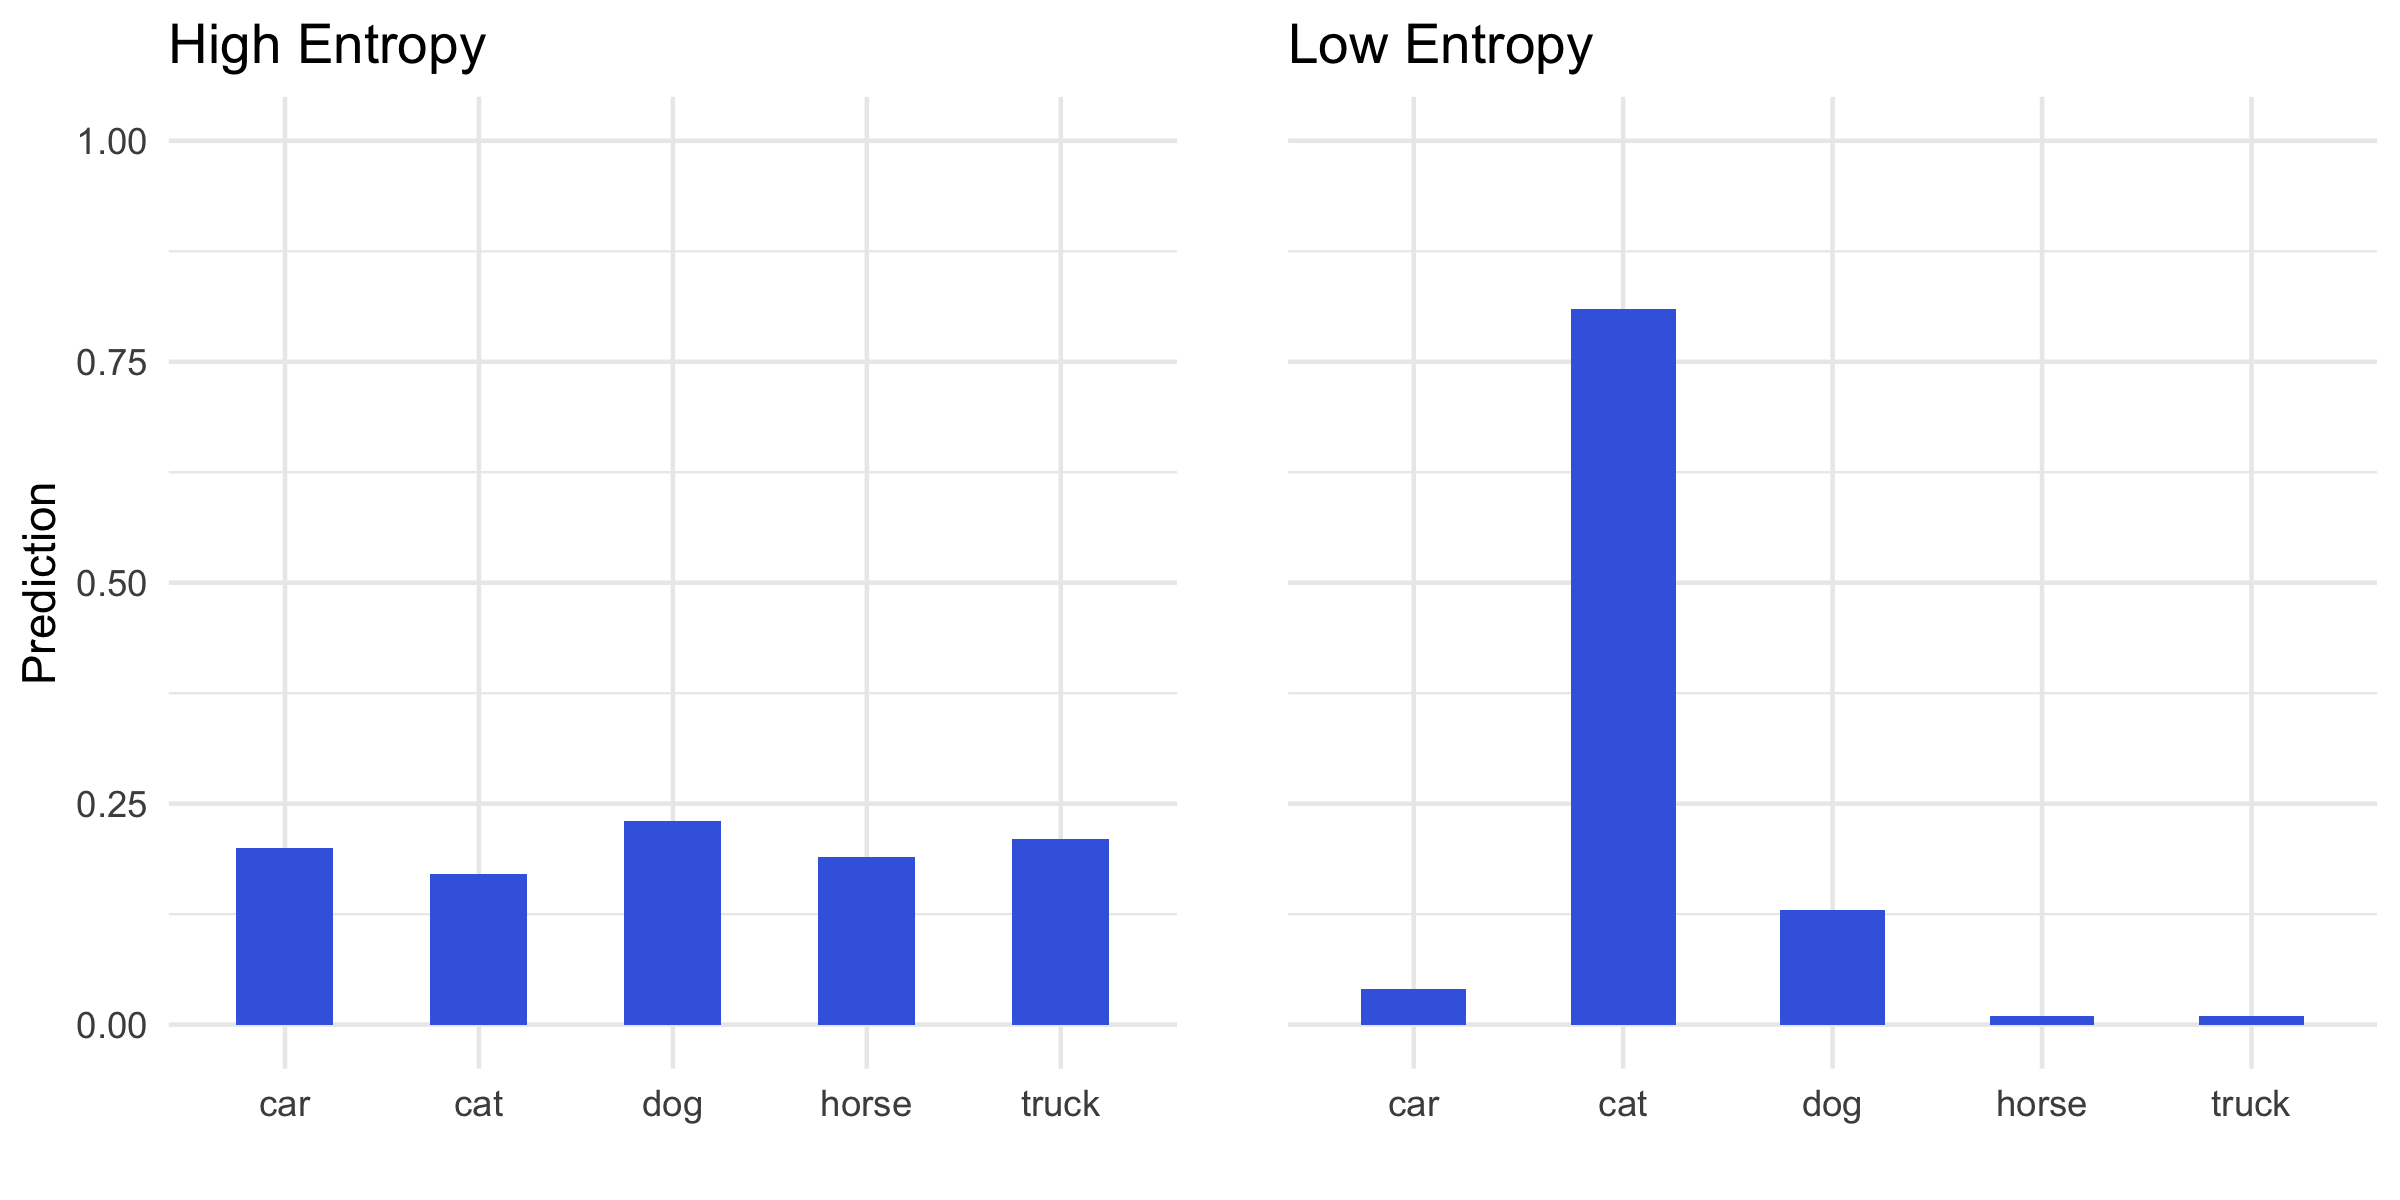
\includegraphics[scale=0.18]{high_vs_low_entropy.png}
        \caption{High vs. low entropy}
        \label{fig:high_vs_low_entropy}
\end{figure}

Therefore, our first approach is to flip the labels of the samples with a high entropy because they are the ones that are more likely to be misclassified. The structure that this algorithm follows is the next one:% and the code is shown in \autoref{listing:entropy_label_flipping_code}:
\begin{enumerate}
        \item Initialize empty lists to store the indices of the samples of the source class and the entropy associated with each sample.
        \item Iterate through the local model's samples using the DataLoader\footnote{A "DataLoader" in PyTorch refers to a utility class that simplifies the process of loading and managing data for training and testing machine learning models.}.
                \begin{enumerate}
                        \item For each sample, we have to check if the sample's label is the source class's label. If it is, we append its index in the list. Since we iterate through batches of samples, it is important to keep the absolute index and not the relative one.
                        \item Then, we introduce the samples into a tensor so we can predict the output the model would return.
                        \item To obtain this output, we call a function that predicts the output of the model.%the \textit{model(data\_source\_batch)} function.
                        \item After that, we must transform the output to NumPy\footnote{NumPy is a fundamental package in the Python programming language used for numerical computations and data manipulation. It provides support for working with large, multi-dimensional arrays and matrices, along with an extensive collection of mathematical functions to operate on these arrays efficiently.} format so we can calculate the entropy.
                        \item Finally, we compute the entropy of the sample and store it in a list.
                \end{enumerate}
        \item We merge the indices and entropies lists into a single list.
        \item The next step is sorting the list by \textbf{highest entropy}.
        \item We select the top 50\% of the list.
        \item We sort it again by index, so we can flip the labels of the samples in the correct order as we iterate in the following step.
        \item To iterate through the samples in the local dataset, we create a \textit{index\_label\_flip()} function %, shown in \autoref{listing:index_label_flip_code} 
        in order to overcome the problem with the main flipping function mentioned in Section \ref{sec:standard_label_flipping}. This function works as follows:
                \begin{enumerate}
                        \item The function receives the dataset, the sorted indices and entropies list, and the target class (its ID).
                        \item It begins by the creation of an empty list to store the poisoned data.
                        \item Then, it iterates through the dataset.
                        \item For each sample, it checks if the sample's index is in the sorted indices list.
                        \item If it is, it appends a structure with the data of the sample and the target class's label to the poisoned data list.
                        \item If it is not, it appends a structure with the data of the sample and the original label to the poisoned data list.
                        \item Finally, it returns the poisoned data list.
                \end{enumerate}
        \item Next, we create a new DataLoader object with the poisoned dataset, ready to be used to train the local model.
        \item Finally, we increment a counter that keeps track of the number of attacks performed and print the information about the attack.
\end{enumerate}


It is important to note that the iterations through the DataLoader are not deterministic if the \textit{shuffle} parameter is set to true because each time we iterate through the DataLoader, the samples are shuffled. Our solution is to set the parameter to false before the first access so we can keep the indices of the samples in the same order to flip them. Then, after the dataset poisoning is completed, as we create the new DataLoader, we set the parameter to true again so the model does not learn the order of the samples.








This attack's structure sets the base that is used for the rest of the attacks. Therefore, the process is almost the same.

%%%%%%%%%%%%%%%%%%%%%%%%%%%%%%%%%%%%%%%%%%%%%%%%%%%%%%%%%%%%%%%
\subsection{Closeness-based label flipping}\label{sec:closeness_label_flipping}
The second proposed algorithm uses the concept of sample closeness, which serves as a metric to determine how closely a given sample aligns with classification as either the source class or the target class. \autoref{fig:high_vs_low_closeness} shows the clear difference between a high and low closeness. The samples with a high closeness are the ones that are likely to be classified as either the source or the target class, while the samples with a low closeness are the ones that are more likely to be classified as one of them.

\begin{figure}[h!]
        \centering
        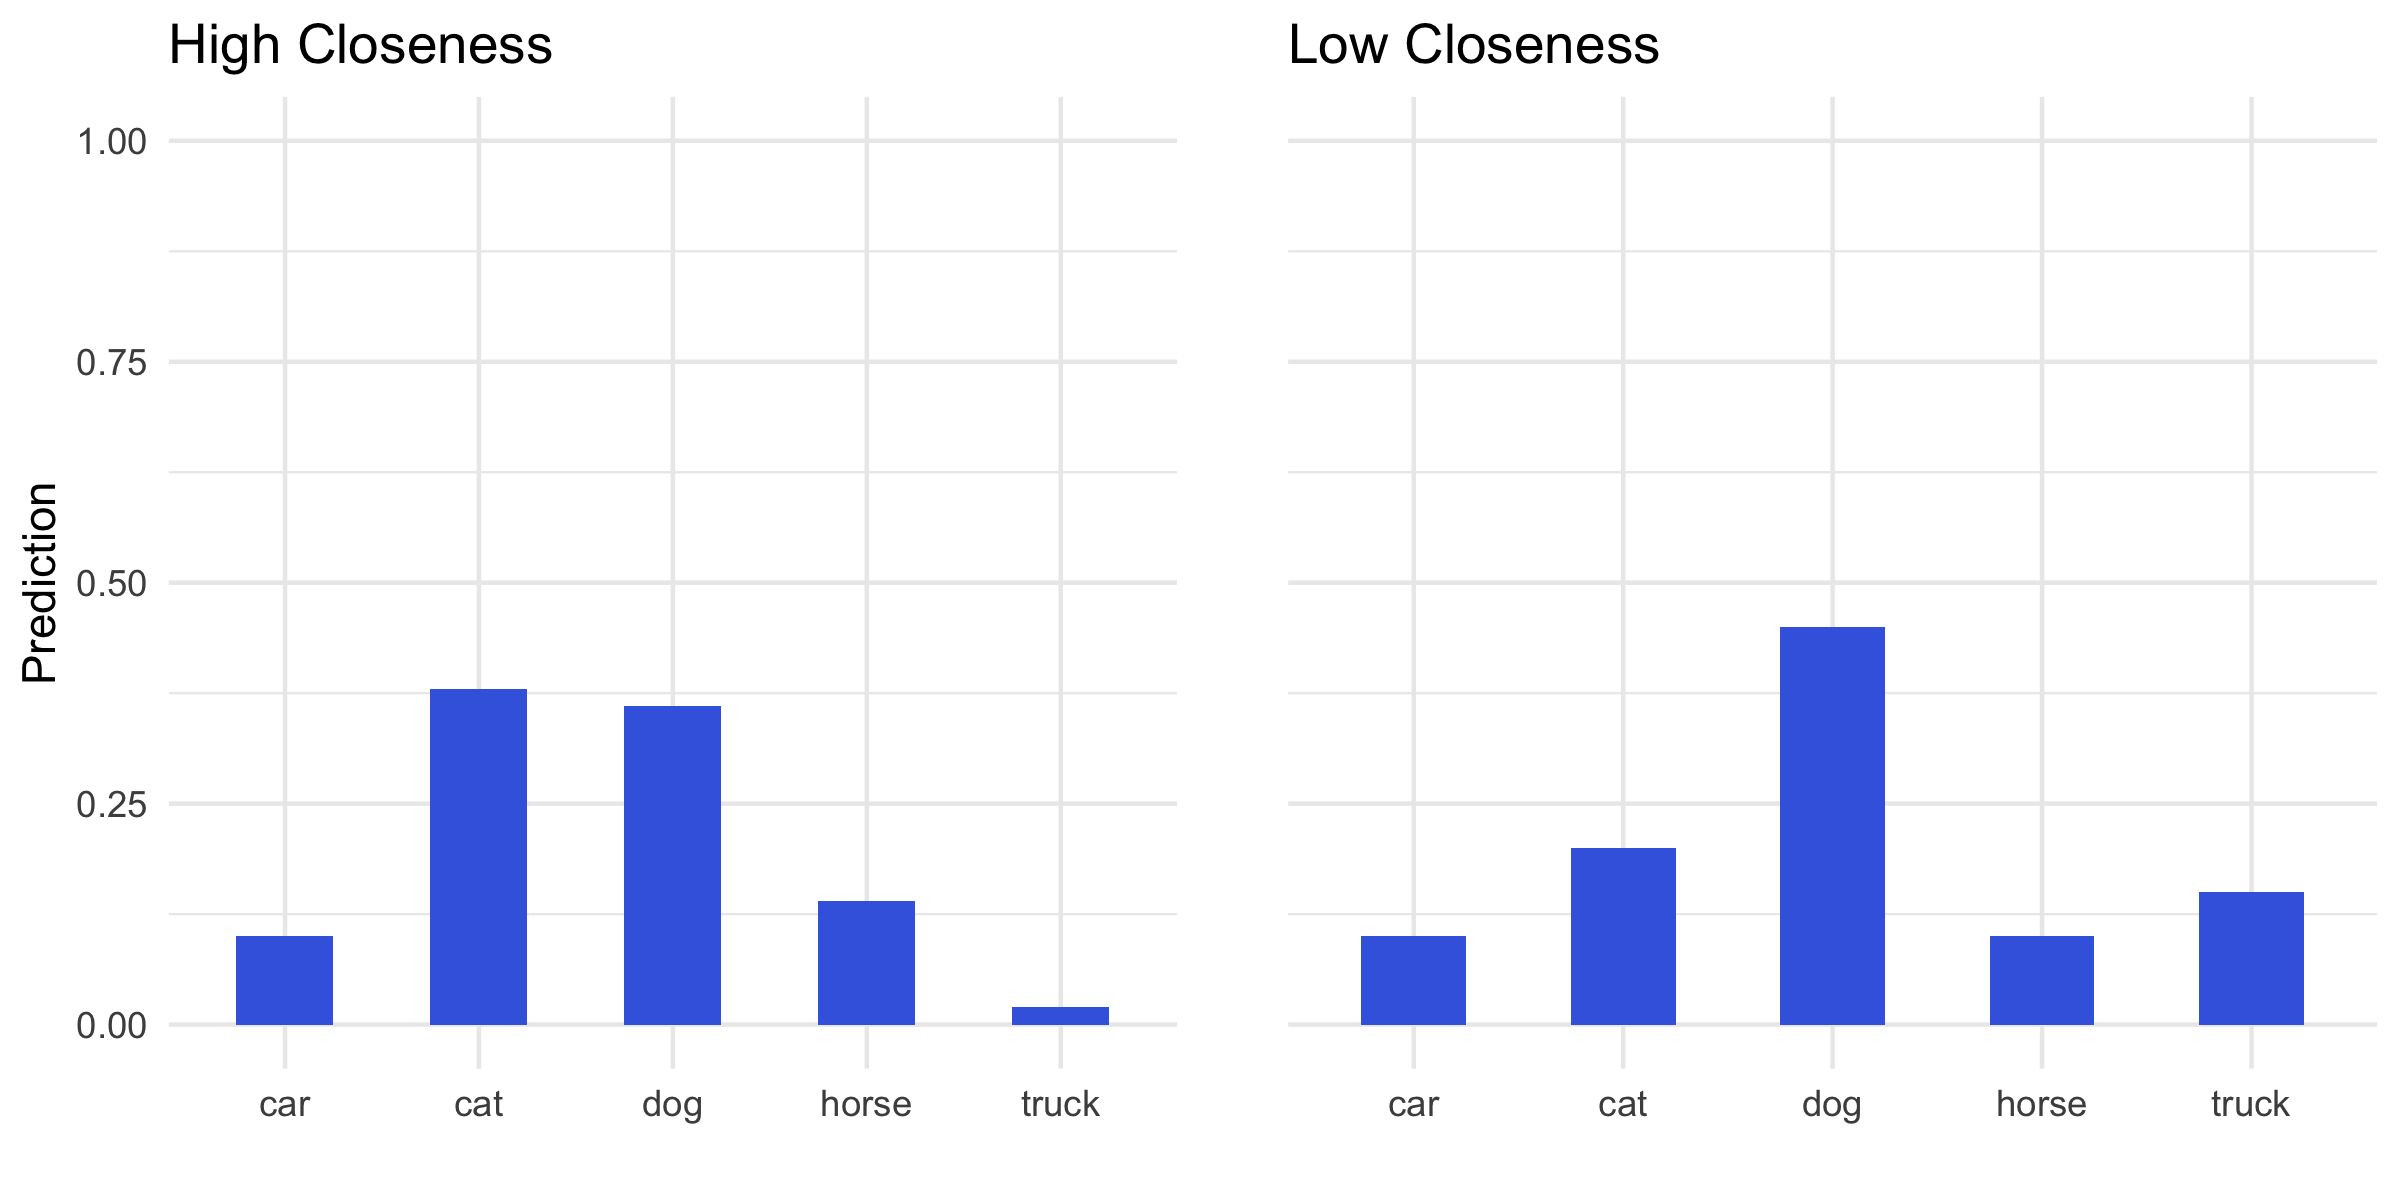
\includegraphics[scale=0.18]{high_vs_low_closeness.png}
        \caption{High vs. low closeness between classes \textit{dog} and \textit{cat}}
        \label{fig:high_vs_low_closeness}
\end{figure}

Hence, our strategy involves flipping the labels of samples exhibiting high closeness, as they are more likely to suffer potential misclassification. Another reason to choose high closeness is that the samples that have the higher closeness between the source and the target classes, may be also the ones more difficult to classify for the other peers. That could be, a dog with a short snout and hairy limbs that at first sight could be thought of as a cat.
The algorithm follows the subsequent structure, summarized since the logic is highly similar to the one explained in Section \ref{sec:entropy_label_flipping}:% and the corresponding code is provided in \autoref{listing:closeness_label_flipping_code}:
\begin{enumerate}
        \item Inside the main loop, iterating through the DataLoader, instead of calculating the entropy, we calculate the closeness between the source and the target class of the sample. This is done by calculating the absolute difference between the output of the model for the source class and the target class. The output is obtained by calling the prediction function, as it was for the entropy solution.
        \item The following steps remain unchanged.
\end{enumerate}






%%%%%%%%%%%%%%%%%%%%%%%%%%%%%%%%%%%%%%%%%%%%%%%%%%%%%%%%%%%%%%%
\subsection{Adaptive label flipping}\label{sec:adaptive_label_flipping}
The idea behind this approach is to use the previous two algorithms to create a more sophisticated and effective attack. The difference resides in the fact that, instead of using a fixed number of samples to flip, we will flip a percentage of the samples depending on how far the global model has been refined, taking into account the global rounds. The rationale behind this is that, since the global model is initialised randomly, the first updates computed by peers are inherently more diverse and thus, more susceptible to attacks. The closer the model is to convergence, the more similar will be the updates of honest peers and, stealthier attacks will be more beneficial, so less labels are flipped. The algorithm follows the subsequent structure, summarized since the logic is highly similar to the one explained in Section \ref{sec:entropy_label_flipping}:% and the corresponding code is provided in \autoref{listing:adaptive_label_flipping_code}:
\begin{enumerate}
        \item Before the main loop, we set an if statement to check if the global rounds are greater than the first defined segment. If they are, the loop will be the same as for either the closeness-based or the entropy-based label flipping algorithm. 
        \item Outside the loop, we will select the number of labels to flip depending on the global rounds. The idea is to flip a percentage of the samples that is inversely proportional to the global rounds. This means that, as the global rounds increase, the percentage of samples to flip decreases.
        \item If the current global round resides on the first segment, the code will be the same as for the standard label flipping algorithm. This means that all the source class labels will be flipped to the target class label.
\end{enumerate}



\newpage